\documentclass[10 pt]{article}
\usepackage{tikz}
\usetikzlibrary{arrows}
\usepackage[margin=0.5 in]{geometry}
\usepackage[utf8]{inputenc}
\usepackage{tabu}
\usepackage{color}
\usepackage{xcolor}
\usepackage{listings}
\usepackage{enumitem}
\usepackage{multicol}
\setlength{\columnsep}{1cm} 
\title{\textbf {Estructuras de Datos 1 - ST0245\\Segundo Parcial Grupo 033 (Martes)}}
\author{Nombre ..............................\\
		Departamento de Informática y Sistemas\\
		Universidad EAFIT\\}
\date{Mayo 07 de 2019}
\begin{document}
\lstdefinestyle{customc}{
	language=Java, 
	numbers=left, 
	showspaces=false,
    showstringspaces=false, 
    tabsize=2, 
    breaklines=true,
    xleftmargin=5.0ex,
}
\lstset{escapechar=@,style=customc, numbers=left, stepnumber = 1} 
\maketitle
\textbf{En las preguntas de selección múltiple, una respuesta incorrecta tendrá
una deducción de 0.2 puntos en la nota final. Si dejas la pregunta sin
responder, la nota será de 0.0. Si no conoces la respuesta, no adivines.}

\begin{multicols}{2}
Para propósitos de este parcial, se considerará esta implementación de un árbol binario y un recorrido.
{\footnotesize
\begin{lstlisting}
class BNode{ //Arbol binario
  BNode izq;
  BNode der;
  int val;
}
void preorden(BNode nodo){ //Recorrido
  if(nodo != null){
    System.out.println(nodo.val);
    preorden(nodo.izq);
    preorden(nodo.der);  
  }
}
\end{lstlisting}
}
	\section{Árboles binarios de búsq. 30\%}
	
	\begin{center}
		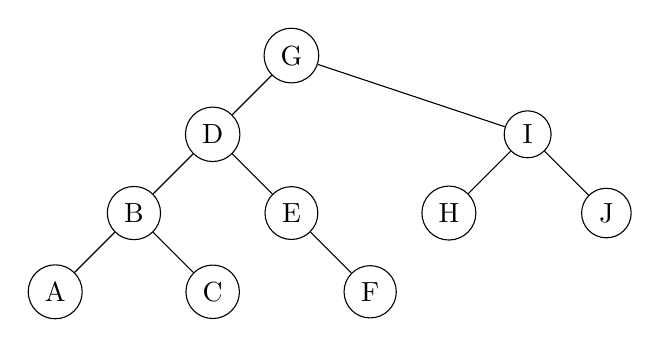
\begin{tikzpicture}
		
		\tikzset{vertex/.style = {shape=circle,draw,minimum size=1.5em}}
		\tikzset{edge/.style = {-,> = latex'}}
		\node[vertex] (G) at (0,0)  {G};
		\node[vertex] (I) at (3,-1)  {I};
		\node[vertex] (H) at (2,-2)  {H};
		\node[vertex] (J) at (4,-2)  {J};
		\node[vertex] (D) at (-1, -1) {D};
		\node[vertex] (E) at (0, -2) {E};
		\node[vertex] (F) at (1, -3) {F};
		\node[vertex] (B) at (-2, -2) {B};
		\node[vertex] (C) at (-1, -3) {C};
		\node[vertex] (A) at (-3, -3) {A};
		%edges
		\draw[edge] (G) to (D);
		\draw[edge] (D) to (B);
		\draw[edge] (D) to (E);
		\draw[edge] (E) to (F);
		\draw[edge] (B) to (A);
		\draw[edge] (B) to (C);
		\draw[edge] (G) to (I);
		\draw[edge] (I) to (H);
		\draw[edge] (I) to (J);
		\end{tikzpicture}
	\end{center}
	Dada la siguiente lista de enteros, ubica los números en el árbol anterior, de tal manera que el árbol final sea un árbol binario de búsqueda: 
	$7, 9, 10, 8, 4, 5, 6, 2, 1, 3$
	\begin{enumerate}[label=\alph*)]
		\item (10\%) ¿Cuáles elementos van en cada letra si se insertan en el orden dado anteriormente?
		\begin{enumerate}[label=\roman*)]
			\item $A = 1, B = 2, C = 3, D = 4, E = 5, F = 6, G = 7, H = 8, I = 9, J = 10$.
			\item $A = 4, B = 5, C = 6, D = 7, E = 8, F = 9, G = 1, H = 10, I = 2, J = 3$.
			\item $A = 7, B = 8, C = 9, D = 10, E = 1, F = 2, G = 3, H = 4, I = 5, J = 6$.
			\item $A = 7, B = 8, C = 9, D = 10, E = 1, F = 2, G = 3, H = 4, I = 5, J = 6$.
		\end{enumerate}
		\item (10\%) ¿Cuál sería el recorrido pre-orden del árbol anterior, asumiendo que siempre se visita primero la hoja de la izquierda?
		\begin{enumerate}[label=\roman*)]
			\item $G, D, B, A, C, E, F, I, H, J$
			\item $A, B, C, D, E, F, G, H, I, J$
			\item $B, C, D, E, F, G, H, I, J, A$
			\item $A, C, B, D, I, J, H, E, F, G$
		\end{enumerate}
		\item (10\%) ¿Cuál es la complejidad asintótica, en el peor de los casos, de encontrar una clave (número) en un árbol binario de búsqueda de $n $ nodos?
		\begin{enumerate}[label=\roman*)]
			\item $O(n)$
			\item $O(\log(n))$
			\item $O(n^2)$
			\item $O(1)$
		\end{enumerate}
	\end{enumerate}
\section{Pilas 20\%}
El método \texttt{push(i)} ingresa el elemento $i$ al tope de la pila. El método \texttt{pop()} retira
el elemento en el tope de la pila y retorna su valor. Considere el siguiente método:
\begin{lstlisting}
void metodo(Stack<Integer> s){
  for(int i = 10; i >= 0; i--){
    if(i % 2 == 0){
      s.push(i);    
    }  
  }
  System.out.print(s.pop());
  while(s.size() > 0){
    System.out.print(" " + s.pop());  
  }
}
\end{lstlisting}
\begin{enumerate}[label=\alph*]
\item (10\%) ¿Cuál es la salida del método anterior?
\begin{enumerate}[label=(\roman*)]
\item 10, 8, 6, 5, 4, 2, 0
\item 2, 4, 6, 8, 10
\item 1, 2, 3, 4, 5, 6, 7, 8, 9, 10
\item 0, 2, 4, 6, 8, 10
\end{enumerate}
\item (10\%) ¿Cuál es la complejidad asintótica, en el peor de los casos, de añadir un nuevo elemento al tope de una pila que contiene $n$ elementos?
\begin{enumerate}[label=(\roman*)]
\item $O(1)$
\item $O(n)$
\item $O(n \log n)$
\item $O(n^2)$
\end{enumerate}
\end{enumerate}
\section{Colas 10\%}
El método \texttt{add(i)} agrega el elemento $i$ al inicio de la cola. El método \texttt{poll()} retira el elemento al final de la cola y retorna su valor. Considere el siguiente método:
\begin{lstlisting}
void metodo(Queue<Integer> q){
  for(int i = 2; i * i <= 25; i++){
    q.add(i);  
  }
  System.out.print(q.poll());
  while(q.size() > 0){
    System.out.print(" " + q.poll());
  }
}
\end{lstlisting}
\begin{enumerate}[label=\alph*]
\item (10\%) ¿Cuál es la salida del algoritmo anterior?
\begin{enumerate}[label=(\roman*)]
\item Los enteros positivos menores que 26 en orden ascendente.
\item Los enteros positivos menores que 26 en orden descendente.
\item 2, 3, 4, 5
\item 5, 4, 3, 2
\end{enumerate}

\end{enumerate}

	\section{Arboles N-arios 20\%}
	La siguiente es una implementación de árbol n-ario.
	\begin{lstlisting}
	class Nodo {
		public int id;
		public int valor;
		public LinkedList<Nodo> hijos;
	}
	\end{lstlisting}
	Hoy, Liko y Kefa, en clase de Estructura de Datos 1, aprendieron que con los árboles $n$-arios se pueden hacer muchísimas operaciones, tales como encontrar el tamaño de un sub-árbol, calcular la suma de los elementos en un sub-árbol, etc. Muchas de estas operaciones son realmente fáciles para Liko; sin embargo, hay una --en especial-- difícil para Kefa. Para Kefa es difícil escribir un programa que calcule la suma de los elementos de los sub-árboles. Liko ha escrito un programa para calcular la suma de los elementos en los sub-árboles para enseñarle a Kefa e intencionalmente ha omitido una parte para asegurarse que, si Kefa entiende el código, él sea capaz de encontrar el error. ¿Podrías ayudarles a Kefa a encontrar el error, por favor? Para propósitos de este ejercicio, Liko se ha asegurado que el árbol dado tiene exactamente $n$ nodos, y que al método \texttt{suma} se le pasa la raíz del árbol y un arreglo con $n$ ceros.
	\begin{lstlisting}
	void suma(Nodo raiz, int[] suma){
	  if(raiz.hijos == null || raiz.hijos.size() == 0){
	    suma[raiz.id] = raiz.valor;
	    return;  
	  }
	  suma[raiz.id] = raiz.valor;
	  
	  for(Nodo e: raiz.hijos){
	      suma(e, suma);
	      suma[..........] = suma[e.id] + suma[raiz.id]; 
	  }
	}
	\end{lstlisting}
	\begin{enumerate}[label=\alph*)]
		\item (10\%) Completa, por favor, la línea 10 ............
		\item (10\%) ¿Cuál es la complejidad asintótica, en el peor de los casos, del código anterior?
		\begin{enumerate}[label=\roman*)]
			\item $T(n) = T(n-1) +   c$, que es $O(n)$
			\item $T(n) = 4.T(n/2) + c$, que es $O(n^2)$
			\item $T(n) = 2.T(n-1) + c$, que es $O(2^n)$
			\item $T(n) = n.T(n-1) + c$, que es $O(n!)$
		\end{enumerate} 
	\end{enumerate}
	\section{Grafos No Dirigidos 20\%}
	\begin{center}
		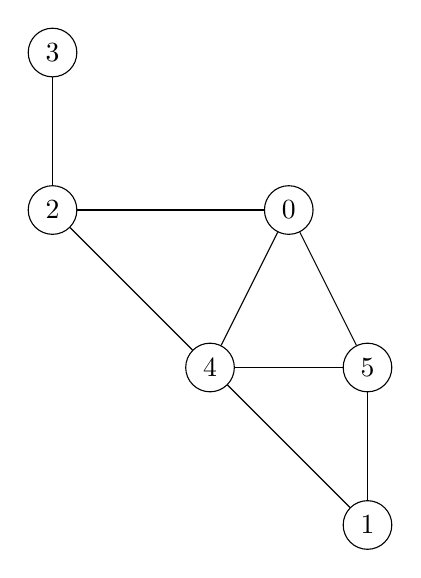
\begin{tikzpicture}
		
		\tikzset{vertex/.style = {shape=circle,draw,minimum size=1.5em}}
		\tikzset{edge/.style = {-,> = latex'}}
		\node[vertex] (0) at (0,0)  {0};
		\node[vertex] (5) at (1,-2)  {5};
		\node[vertex] (4) at (-1,-2)  {4};
		\node[vertex] (1) at (1,-4)  {1};
		\node[vertex] (2) at (-3, 0) {2};
		\node[vertex] (3) at (-3, 2) {3};
		%edges
		\draw[edge] (0) to (4);	
		\draw[edge] (0) to (5);
		\draw[edge] (5) to (4);
		\draw[edge] (5) to (1);
		\draw[edge] (4) to (1);
		\draw[edge] (4) to (2);
		\draw[edge] (0) to (2);
		\draw[edge] (2) to (3);
		\end{tikzpicture}
	\end{center}
	\begin{enumerate}[label=\alph*)]
		\item (10\%) ¿Cuál es un recorrido de \emph{búsqueda primero en profundidad} del grafo anterior, si como nodo inicial se toma el nodo 1?
		\begin{enumerate}[label=\roman*)]
			\item 1, 5, 0, 3, 2, 4
			\item 1, 4, 5, 0, 2, 3
			\item 1, 4, 0, 3, 5, 2
			\item 1, 5, 4, 0, 3, 2
		\end{enumerate}
	    \item (10\%) ¿Cuál es un recorrido de \emph{búsqueda primero en amplitud del grafo anterior}, si se toma como nodo inicial el nodo 1?
	    \begin{enumerate}[label=\roman*)]
	    	\item 1, 4, 5, 0, 2, 3
	    	\item 1, 5, 0, 2, 3, 4
	    	\item 1, 4, 2, 0, 3, 5
	    	\item 1, 3, 0, 4, 5, 2
	    \end{enumerate}
	\end{enumerate}
\end{multicols}
\end{document}